\subsection{Forretningsmodel}
Psykolog Nord er en psykologkæde med 3 afdelinger: en i Aalborg, Aarhus og Odense. De har 3 psykologer:

\begin{itemize}
    \item Katrine Breum Larsen
    \item Miriam Poulsen
    \item Stefan Guldager Boldemann
\end{itemize}

Lige nu er Katrine og Miriam begge tilknyttet afdelingerne i Aalborg og Aarhus, og Stefan er tilknyttet afdelingen i Odense.

Psykolog Nord tilbyder psykologbehandling uden ventetid.
Derfor har de åbent alle 7 dage i ugen fra kl. 9 til 21. De tjener penge på honorarer fra klienter.

De tilknyttede psykologer er ikke ansat af Psykolog Nord, men er partnere.
Derfor skal de ikke betale løn og pension, men derimod har de aftalt, at psykologen modtager halvdelen af betalingen fra klienten.

Firmaet drives af brødrene Anders Mikkelsen og Lasse Kirk, og Lasses kæreste Katrine Breum Larsen.
De har en flad firmastruktur, hvor alle 3 indgår i firmaets ledelse, men Katrine står for den daglige ledelse. 
Firmaet tilhører den basale form fra Mintzbergs fem organisationsformer, og på figur \ref{forretning:organisationsdiagram} kan man se deres virksomhedsstruktur.

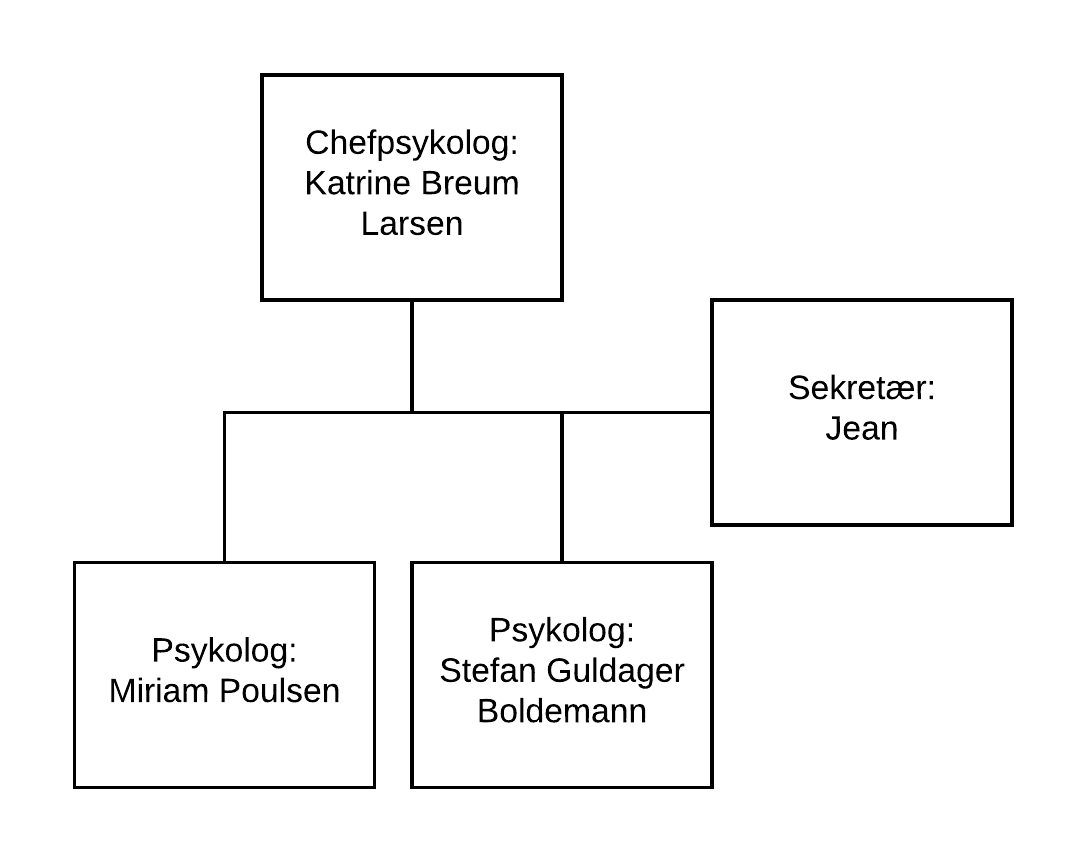
\includegraphics[scale=.8]{OrganisationsDiagram}\label{forretning:organisationsdiagram}